-This chapter will describe how the system will be designed, how the Field of application can be modelled, what functionalities can be planned-

\section{Field of application}
A precise definition of what a system is able to do is only possible when a defining of the situation respectively problem is available. Context of such a definition is the physical environment, questioning which entities are part of the situation, how are they interacting, and which functionalities are they using for that. But also the participating actors and their use cases must be modelled in order to get an idea of what the user is really needing.

The system which will be conceptualised with this thesis will help field engineers with their work in field dealing with different Sensors. As an concrete example the systems application domain will be structural health monitoring (SHM).The technology of the structural health monitoring helps to avoid damages or unnecessary deconstructions of objects. It is basing on the measurement of changes of the states and behaviour of a material in different domains concerning the buildings structure. For the better understanding, I will explain two different cases: First, a bridge with a high traffic is reaching its final year of its planned life time. Since the engineer cannot be sure, that the condition of the bridge is better then planned and good enough for a longer life time, the bridge has to be closed. The structural health monitoring is following the approach to observe an object over a longer period and performing an automated monitoring, inspection and damage detection. SHM is periodically producing diagnostic on the basis of structural dynamics analysis, recognising material fatigue, non-destructive testing and evaluation and much more over time. A SHM-System implies a sensor network that monitors the described changes using a band of different sensors \citep{worden_overview_2004} \citep{farrar_introduction_2007} \citep{boller_structural_2004}. More detailed descriptions of the used measurements, time-scales and analysis-methods will be explained in the methodical part.

As the best way to introduce to and describe the system, I will follow the procedure of a software development concept which is describing similar information as my approach in modelling, see \citep{gregor_engels_vorlesung_2006}. Such a concept begins with a description of the actual situation, models then the processes and the participating actor with their use cases, and ends up with an approach of necessary functionalities.

\subsection{Model of domain}
The actual Situation is containing five different types of entities and their relationships between each other. Central Object will be a Server which is the communicating node and connected to all other facilities. Those are mainly the sensors themselves. The Sensors cannot exist without an Server being the managing and storing device of each sensor. Nevertheless sensors can also be organised within a sub-network with its own small sub-server. Such a sub-network would be managed as a single sensor. Sensors can be controlled, which means activated and deactivated, by the server. Sensors are either actively sending their data to the server, or the server is requesting their data.

\begin{figure}[H]
	\centering
 	 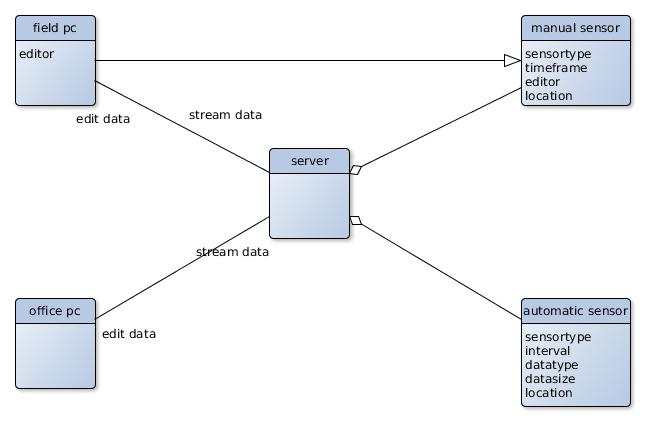
\includegraphics[scale=0.6]{graphics/model_of_issue.jpg} 
	\caption{Model of domain with relevant features. By F. H. Euteneuer 2013}
	 \label{fig:model_domain}
\end{figure}

The Server is connected to a database storing both, metadata of the different sensors, and their measured data. As a viewing device any kind of mobile computer can be connected to the database. Since such a connection will use the TCP/IP protocol, this mobile computer must be connected to the internet. For manual measurements, the mobile device would additionally to the viewing function also provide a data insertion function. Therefore the mobile computer will be treated also as a sensors, it is inheriting the features of the sensor entity.

The office part of the system is represented by the desktop-computer which will form the management basis. additionally to the features of a field computer it is dealing with advanced analysis and also data output in different formats and using different protocols. A real difference between the platforms will not exist, but the usage will be assumed to be different.

The figure \ref{fig:model_domain} is showing an UML Class Diagram representing the explained Entities of the System. It is important to now, that this model is not containing any activity of functionality. It is simply containing the required objects its features and their relationships. 


\subsection{Business processes}
The reason why such a system might be relevant for the future work of field engineers is, that it is following a decision support approach without dealing with a bunch of different unnecessary tools. The system is focussing on the information which are important to have in the field. In the previous chapter I was introducing into the field of domain the system is dealing with. Now I will give an overview about the different processes which the user might perform.

\begin{figure}[H]
	\centering
 	 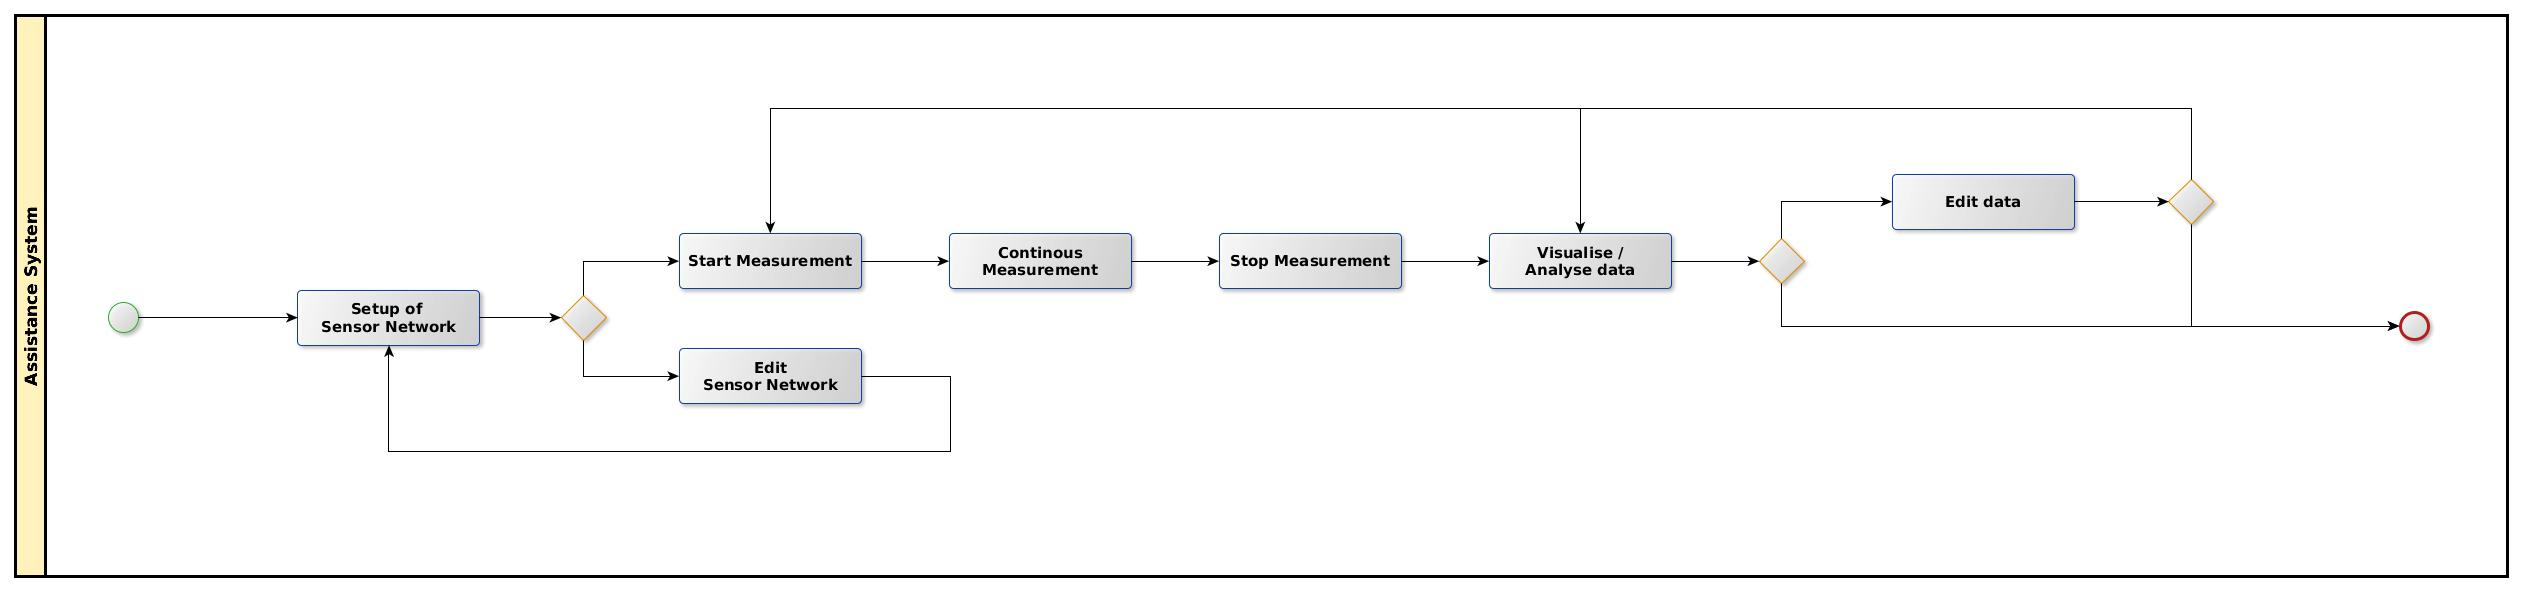
\includegraphics[scale=0.2]{graphics/bpmn_business-processes.jpg} 
	\caption{BPMN (Business Process Model and Notation) Model of relevant general business processes within the system. By F. H. Euteneuer 2013}
	 \label{fig:model_business-processes}
\end{figure}
I have identified three different main actions a user might perform: The manual measurement, the manual editing of measurement results and the automatic measurement. The figure \ref{fig:model_business-processes} is showing an UML Activity Diagram describing the work-flows of the different activities. As drawn in the graphic some actions are causing other.

The Manual Measurement is starting with the pure measurement. After entering the results in the System the validation and a performance of first automatic analysis will be done. This first statistics will be necessary to get information about the quality of the measurements, and they are helping with the decision whether to redo the measurements or to approve them. The system will give advices which measurement might be incorrect.

The user will also have the option to manually edit historical measurements. Therefore one dataset (which is one measurement)has to be selected. Either the user can redo the measurements, and will follow up in the manual measurement work-flow, or the new correct values can been entered by hand.

The automatic measurements are the most important one for the described SHM. The will be the backbone of the system, nevertheless they are using similar functionalities. The user will initially be able to set the sensor network up. Which means to enter metadata about the used sensors like position, reference system, type of sensor, measurement interval, etc. A more detailed description of what is needed for such a setup will follow in the methodical part. After the setup, the user is able to start the measurements with the defined parameter, or the edit the settings.

As a conclusion of this chapter, I would like to point out that this list is only representing functionalities of a basic system, and should not be understood as being complete.


\section{Functionalities}
This chapter will describe what the system should provide to solve the problem and/or make the existing situation better: Which functionalities should be part of the system. To get closer to a possible solution, the different stakeholders and their use cases in the domain of structural health monitoring must be defined and described.

\begin{figure}[H]
	\centering
 	 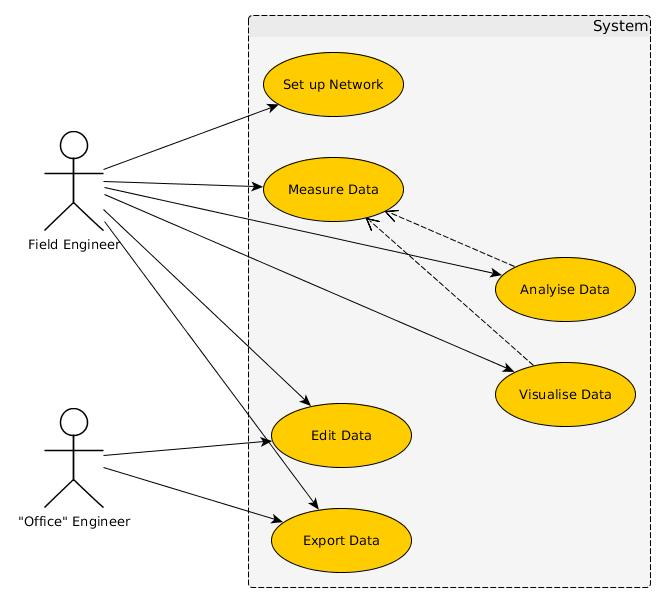
\includegraphics[scale=0.6]{graphics/uml_functionalities.jpg} 
	\caption{UML Use Case Diagram of the described System describing two different users and their use cases. By F. H. Euteneuer 2013}
	 \label{fig:model_functionalities}
\end{figure}

\subsection{Usergroups}
As a main source for information and parameter for the concept of a software, the usergroups are of large importance. I will analyse the involved usergroups and their needs respective expectations to get those information. As the figure \ref{fig:model_functionalities} is already representing, I have identified two main usergroups which might be involved in the processes.

\subsubsection{Field-engineer}
The group of field-engineers can described as the executive persons which are dealing with the direct measurements, observations and setup of an automatic measurement network. This group can be categorised by its technically limits, which are:
\begin{itemize}
\item the small screen-size of the mobile computers (quality of visualisation is limited)
\item the lack of input facilities (e.g. only digital keyboard on a handheld computer)
\item high weight of not handheld instruments (e.g. a conventional laptops too heavy for using while walking/standing)
\end{itemize}
But nevertheless, this usergroup has the most challenging requirements on the system when speaking about visualisation options or analysis computation in advance. It is the central target usergroup for this system, therefore it should fit mostly to its requirements.


\subsubsection{Office-engineer}
Usually the field-engineer and the office-engineer are combined in one person. One part of an observation project is dealing with the field-work, the setup, measurements and maintenance. And the other part is the precise analysis of the data, the post processing and its interpretation. Due to a high quality equipment in the offices, this part is mostly better solvable for a software. Here does not the system has to be restricted by the environment, but the system is making its demands on the technical environment.


\subsection{Use Cases}
The Figure \ref{fig:model_functionalities} is showing the different basic use cases of the described two usergroups. Use cases shown in this figure are representing activities of the user which have to be complete with it own defined target. I want now describe the use cases in detail with further parameter. This is important for the further proceeding of the system conception, because use cases are defining the users interests of a system.

The following part will describe the selected use cases in detail. All the use cases will be described with tables for the textual description which are containing information about the use case goal, the postcondition and further more. For the description of the the chronological task flow of the use cases also a activity diagram will depict each use case.


\subsubsection{Management}
There are several use cases with central management functionalities of the system. Management stands for both, data management and system management.  

First use case within the system is the setting up of the network. It can be understood as the initial task and therefore a kind of a precondition for all other use cases.The table \ref{table:use case description of "Set up network"} is describing central features of this use case. 

The export of the data is another major task within the management field. It could be denoted as the final task interacting with the system. The second table \ref{table:use case description of "Export data"} is showing detailed information about the "Export data" use case.

\begin{table}[H]
\centering
\begin{tabular}{l | p{11cm}}
Name & Set up network\\ \hline 
Usergroup & Field engineer\\ \hline 
Goal & Input all metadata about connected sensors and initialise network\\ \hline 
Precondition & Network physicaly existing and able to correspond with system\\ \hline 
Postcondition & working network with all sensors\\ 
\end{tabular}
\caption{Use Cases tabular description of characteristics} 
\label{table:use case description of "Set up network"}
\end{table}

\begin{table}[H]
\centering
\begin{tabular}{l | p{11cm}}
Name & Export data\\ \hline 
Usergroup & Office Engineer\\ \hline 
Goal & Specify data by parameter and specify oputput format\\ \hline 
Precondition & Spcified data and output format\\ \hline 
Postcondition & complete dataset in specific format offline\\ 
\end{tabular}
\caption{Use Cases tabular description of characteristics} 
\label{table:use case description of "Export data"}
\end{table}

Figure \ref{fig:bpmn_use-case_management} is showing the systems management use cases in a two line activity diagram. The both activity flows do not have any interaction in between, but chronologically must the setup use case performed before the export use case.

The activity flow of the setup use case is showing two main tasks: The database-setup and the input of the sensor-parameter. Those are the central parts and their success or failure is leading to an overall success or failure. An edit of an existing network is leading to a restart of the full procedure. This could be interpreted as an assistant which is leading through the different configurations and is taking care of possible errors.

The export use case is much easier, it is simply the normal flow which is equal to most of the download assistants which can be found online. The only important information about that is the determination of the export datasets time-frame.

\begin{figure}[H]
	\centering
 	 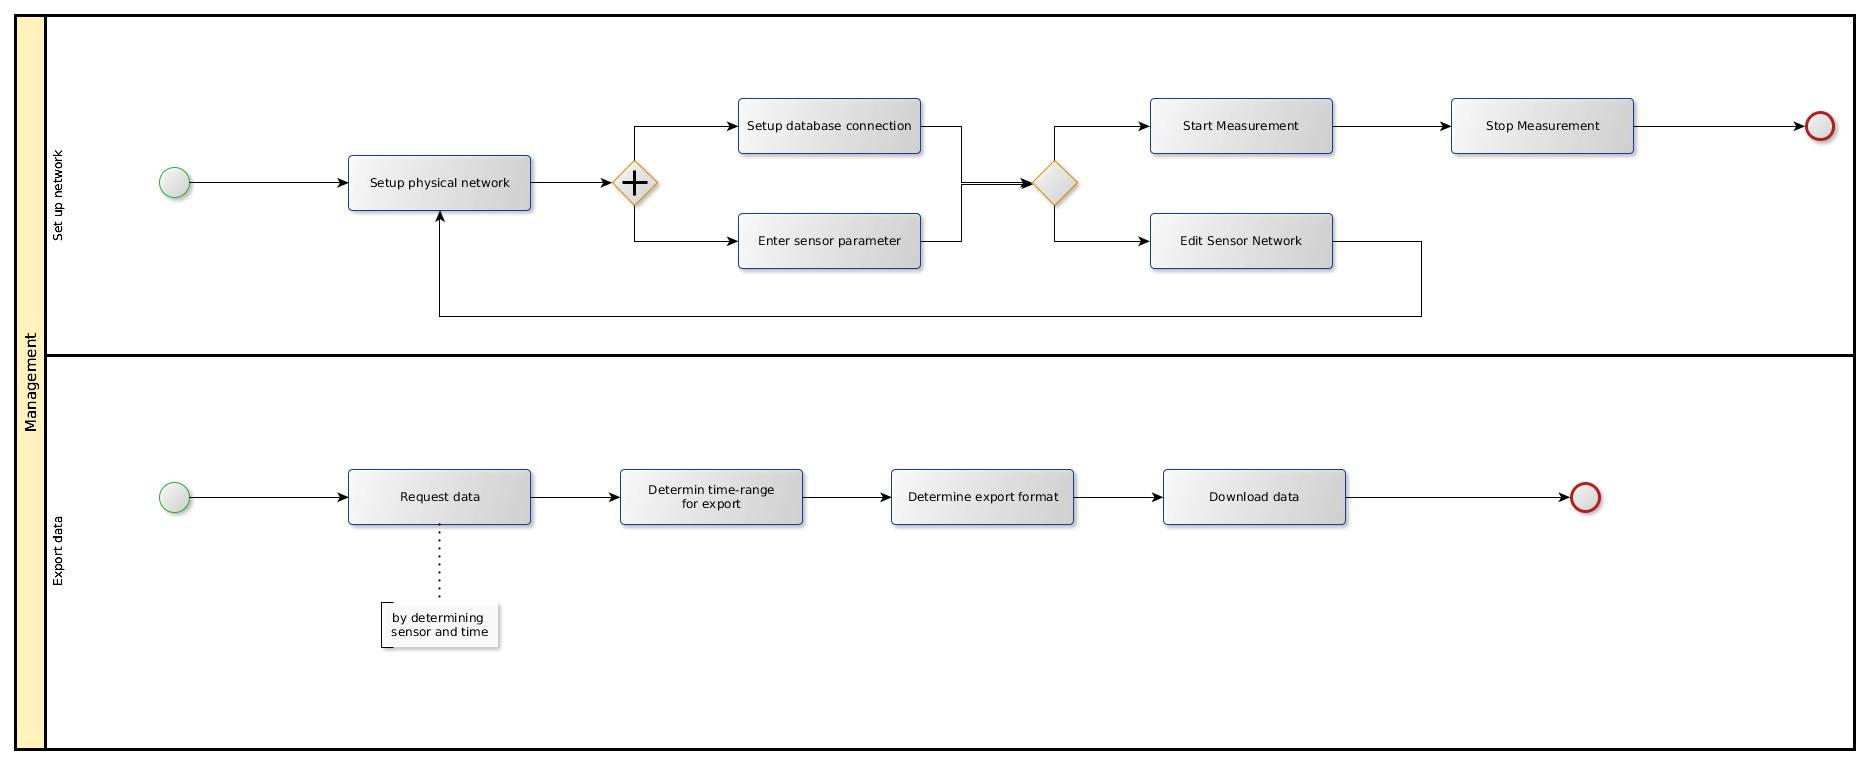
\includegraphics[scale=0.24]{graphics/bpmn_use-cases_management.jpg} 
	\caption{BPMN (Business Process Model and Notation) Model of the use cases describing central management proceedings. By F. H. Euteneuer 2013}
	 \label{fig:bpmn_use-case_management}
\end{figure}


\subsubsection{Measuring}

The measurement part might be the most important one within the system. Central 

\begin{figure}[H]
	\centering
 	 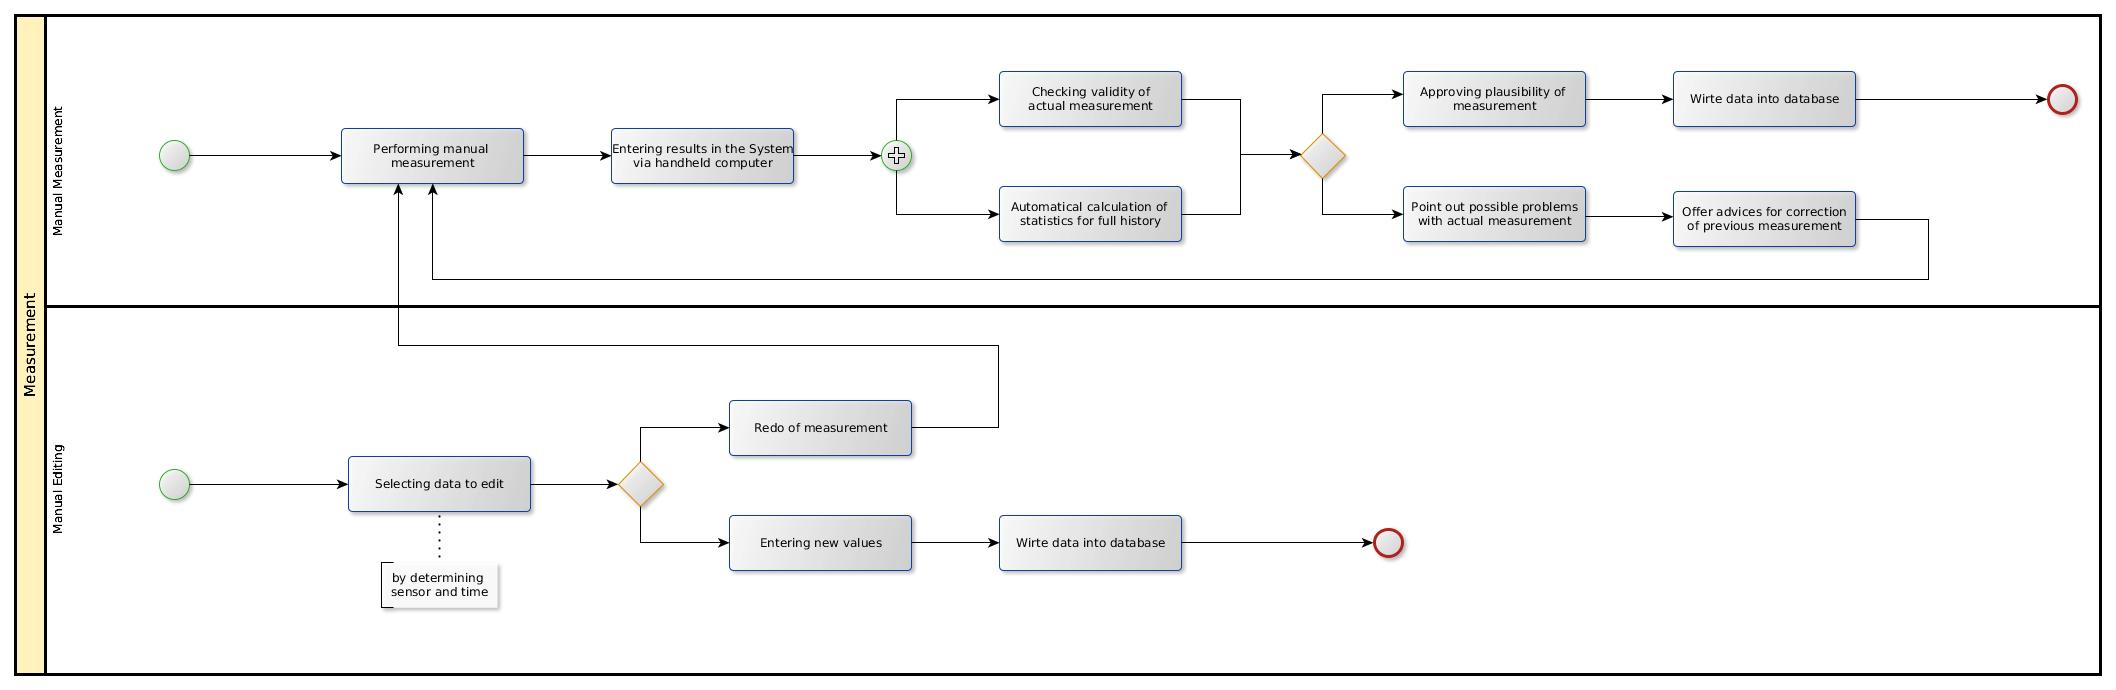
\includegraphics[scale=0.24]{graphics/bpmn_use-cases_measurement.jpg} 
	\caption{BPMN (Business Process Model and Notation) Model of the use cases describing central measuring proceedings. By F. H. Euteneuer 2013}
	 \label{fig:bpmn_use-case_measuring}
\end{figure}

\begin{table}[H]
\centering
\begin{tabular}{l | p{11cm}}
Name & Measure data\\ \hline 
Usergroup & Field engineer\\ \hline 
Goal & Input all data by hand  getting from standalone measurement device\\ \hline 
Precondition & Running system and access to database\\ \hline 
Postcondition & valid data in the database with full set of metadata\\ 
\end{tabular}
\caption{Use Cases tabular description of characteristics} 
\label{table:use case description of "Measure data"}
\end{table}

\begin{table}[H]
\centering
\begin{tabular}{l | p{11cm}}
Name & Edit data\\ \hline 
Usergroup & Office Engineer\\ \hline 
Goal & Spcify data by parameter and inout new values by hand or measurement\\ \hline 
Precondition & Running system and access to database\\ \hline 
Postcondition & changed data in the database with full set of metadata\\ 
\end{tabular}
\caption{Use Cases tabular description of characteristics} 
\label{table:use case description of "Edit data"}
\end{table}


\subsubsection{Analysis}

\begin{figure}[H]
	\centering
 	 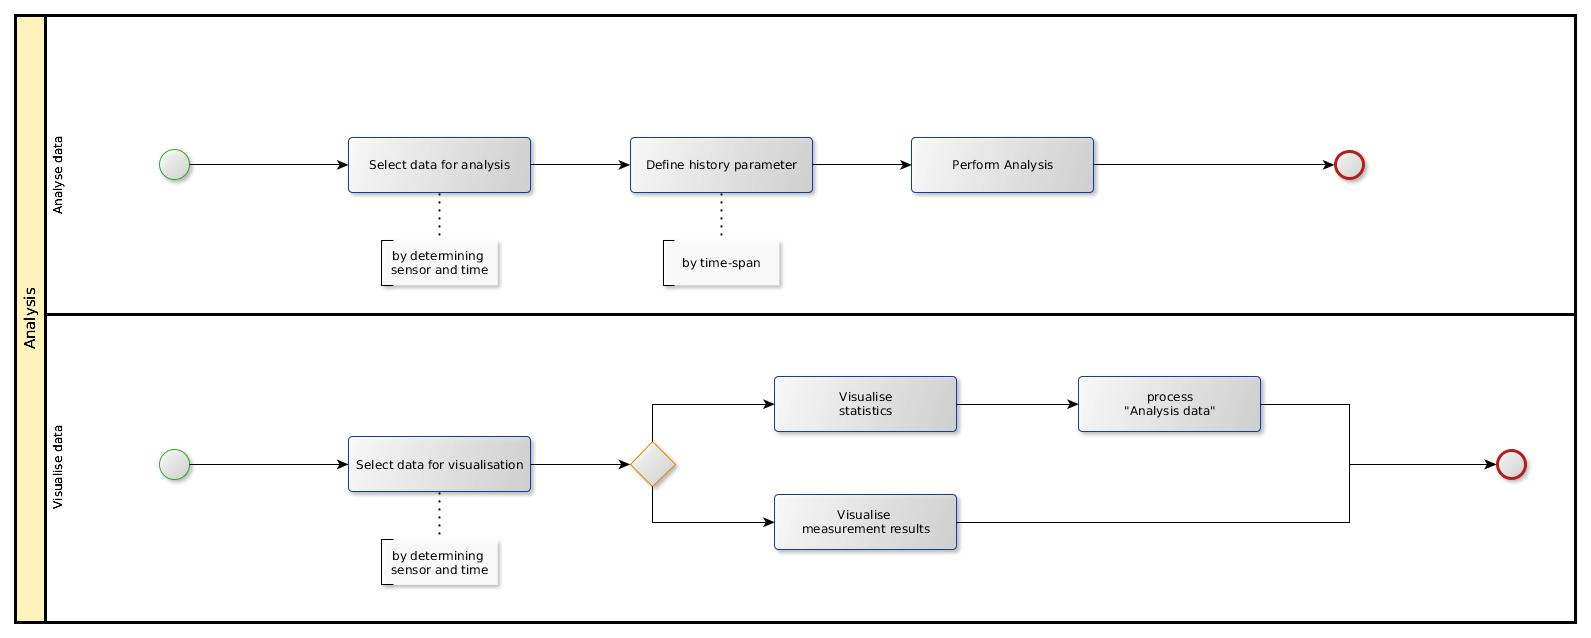
\includegraphics[scale=0.24]{graphics/bpmn_use-cases_analysis.jpg} 
	\caption{BPMN (Business Process Model and Notation) Model of the use cases describing central analysis proceedings. By F. H. Euteneuer 2013}
	 \label{fig:bpmn_use-case_analysis}
\end{figure}

\begin{table}[H]
\centering
\begin{tabular}{l | p{11cm}}
Name & Visualise data\\ \hline 
Usergroup & Field engineer\\ \hline 
Goal & Getting support by visualising measurements and interpretation\\ \hline 
Precondition & Existing meatadat for measurements\\ \hline 
Postcondition & meaningful and „supporting“ graphic\\
\end{tabular}
\caption{Use Cases tabular description of characteristics} 
\label{table:use case description "Visualise data"}
\end{table}

\begin{table}[H]
\centering
\begin{tabular}{l | p{11cm}}
Name & Analyse data\\ \hline 
Usergroup & Field engineer\\ \hline 
Goal & Getting information about validity of data in comparison to historical data\\ \hline 
Precondition & Amount of measurements higher then two\\ \hline 
Postcondition & information about validity of the data\\ 
\end{tabular}
\caption{Use Cases tabular description of characteristics} 
\label{table:use case description of "Analyse data"}
\end{table}





